\chapter{Evaluation}
\label{ch:evaluation}

The goal of this thesis can be summarized as implementing the \ac{SCITE} algorithm with the same solution quality as the reference implementation, but faster. We describe our design choices in the previous chapter \ref{ch:design}, but we also needed to verify that these choices lead to this goal. This chapter describes how we tested the solution quality of \ac{ffSCITE} using the \ac{TOST} procedure \cite{schuirmann1987comparison} and evaluated its performance using the synthesis report, benchmarking, and profiling. 

Before we can discuss the features of the final build of \ac{ffSCITE}, we need to address a general issue: In section \ref{sec:encoding}, we have decided to limit the maximal number of cells and genes that are processable by the compiled design to an arbitrary number. Therefore, we need to decide on a number of cells and genes for our final design. Our final build of \ac{ffSCITE} supports 64 cells and 63 genes, which is equivalent to mutation trees with 64 nodes. This covers all but one of the example datasets that is bundled with the source code of \ac{SCITE} and compiling the design for 128 cells and 127 genes leads to internal compiler errors we were not able to resolve in time. Lastly, targeting 64 cells and 63 genes also leads to reasonable resource usage which we will discuss later. Therefore, we decided to continue with this input size.

In this chapter, we will first discuss the properties that can be evaluated using the final synthesis report, namely the hardware usage and loop characteristics. We are then using this information to predict the performance of the design and benchmark both \ac{SCITE} and \ac{ffSCITE} to verify this prediction and to evaluate the throughput difference between them. Lastly, we evaluate the solution quality of \ac{ffSCITE}, for which we have to introduce and execute a statistical test. The most important results of these sections are listed in table \ref{tab:quickfacts} for quick look-up.

\begin{table}
    \centering
    \begin{tabular}{r|l}
        \textbf{Metric}                     & \textbf{Value} \\
        \hline
        Max. no. of cells                   & 64 \\
        Max. no. of genes                   & 63 \\
        \hline
        Clock frequency                     & 295.83 MHz \\
        Macro-pipeline capacity             & 6 states \\
        Device utilization (Kernels + DSP)  & 69\% \acsp{LUT} \\
        Predicted throughput                & 577.79 ksteps/s \\
        Measured throughput                 & 566.72 ksteps/s \\
        Maximum speedup                     & 8.63 \\
        \hline
        \ac{FPGA}                           & Intel Stratix 10 GX 2800 \\
        Board                               & Bittware 520N \\
        oneAPI/SYCL version                 & 2022.2.0 Build 133.4 \\
        Quartus version                     & 20.4.0 Build 72 Pro \\
        BSP version                         & 20.4.0\_hpc \\
    \end{tabular}
    \caption{Quick facts about the final \ac{ffSCITE} build.}
    \label{tab:quickfacts}
\end{table}

\section{Hardware usage}

Tables \ref{tab:abs-usage} and \ref{tab:rel-usage} list the hardware usages of the different kernels for our target \ac{FPGA} and input sizes. The overall design is very logic-intensive, which makes sense since most of the work is done with custom logic and very few floating-point operations. Of all individual components indicated in the design schematic (Figure \ref{fig:design_schematic}), the tree score mapping loop is the heaviest and makes up roughly 37.7\% and 37.5\% of the entire design's \ac{LUT} and \ac{FF} usage, respectively. This makes sense since it is a three-dimensional loop where the inner-most loop is completely unrolled (i.e. unroll factor 64) and the middle loop is eight times partially unrolled, as we have discussed in section \ref{sec:scoring}. Therefore, the inner loop's body is replicated 512 times, which leads to the reported resource usage. The next-biggest component is the change proposer with 33.3\% and 25\% of the design's \ac{LUT} and \ac{FF} usage, respectively. This resource usage is independent of the input size since it is dominated by the \ac{URNG} executions which involve a 64-bit integer multiplication and remainder operation; Compiling the design for smaller input sizes yields similar resource usages for the change proposer.

It may be possible to further unroll the middle loop of the tree score mapping loop and double its potential throughput and hardware usage, and an extension to bigger inputs may be possible if the compiler issues were resolved. However, experience has shown us that designs with a total logic usage over 75\% start to run into issues regarding compilation times and clock frequencies. Therefore, we decided to settle with this configuration. It is however impossible to replicate the entire design another time to double the potential performance.

\begin{table}
    \centering
    \begin{tabular}{l|l|l|l|l|l}
        &                           \textbf{LUTs}&      \textbf{FFs} &      \textbf{RAMs} & \textbf{MLABs} &    \textbf{DSPs} \\
        \hline
        Pipe resources &            90 &                1.9k &              0  &            0  &                0 	\\
        IO-Kernel &                 12.3k &             3.9k &              180 &           431 &               1.5 \\
        Tree Scorer &               537.4k &            817.7k &            2.0k &          1.6k &              340.5  \\
        - Find Parent Loop &        34.1k &         	48.2k &	            22 &            46 &                0 \\
        - Tree Update Loop &        54.1k &             61.5k &             131 &           32 &                0 \\
        - Tree Score Mapping Loop & 313.4k &            439.9k &            332 &           262 &               72 \\
        - Tree Score Reduction Loop& 31.5k &            70.3k &             309 &           32 &                0 \\
        Change Proposer &           274.1k &            307.4k &            114 &           299 &               40.5 \\
        \hline
        \textbf{Kernels} &          \textbf{843.8k} &   \textbf{1.2M} &     \textbf{2.4k} &	\textbf{2.4k} &     \textbf{382.5} \\
        \textbf{Static Partition} & \textbf{455.2k} &   \textbf{910.5k} &   \textbf{2627} &	\textbf{0} &        \textbf{1.0k}	
    \end{tabular}
    \caption{Hardware usage of \ac{ffSCITE} in absolute numbers, supporting up to 64 cells and 63 genes, as reported in the ``Area Analysis'' report.}
    \label{tab:abs-usage}
\end{table}

\begin{table}
    \centering
    \begin{tabular}{l|l|l|l|l|l}
        &                               \textbf{LUTs}&  \textbf{FFs} &  \textbf{RAMs} & \textbf{MLABs} &    \textbf{DSPs} \\
        \hline
        Pipe resources &                <1\% &          <1\% &          0\% &           0\% &               0\%	\\
        IO-Kernel &                     1\% &           1\% &           2\% &           <1\% &              <1\% \\
        Tree Scorer &                   29\% &          22\% &          17\% &          2\% &               6\% \\
        - Find Parent Loop &            2\% &           1\% &           <1\% &          <1\% &              0\% \\
        - Tree Update Loop &            3\% &           2\% &           1\% &           <1\% &              0\% \\
        - Tree Score Mapping Loop &     17\% &          12\% &          3\% &           0\% &               1\% \\
        - Tree Score Reduction Loop&    2\% &           2\% &           3\% &           <1\% &              0\% \\
        Change Proposer &               15\% &          8\% &           1\% &           <1\% &              1\% \\
        \hline
        \textbf{Kernels} &              \textbf{45\%} & \textbf{32\%} & \textbf{20\%} & \textbf{3\%} &      \textbf{7\%} \\
        \textbf{Static Partition} &     \textbf{24\%}&  \textbf{24\%} & \textbf{22\%} & \textbf{0\%} &      \textbf{18\%}	
    \end{tabular}
    \caption{Hardware usage of \ac{ffSCITE} relative to the resources available on Intel Stratix 10 GX 2800 \acp{FPGA}, supporting up to 64 cells and 63 genes, as reported in the ``Area Analysis'' report.}
    \label{tab:rel-usage}
\end{table}


\section{Throughput prediction}

\begin{table}
    \centering
    \begin{tabular}{l|l|l}
        \textbf{Kernel/Loop} & \textbf{\acs{II}} & \textbf{No. of iterations (unrolled)} \\
        \hline
        IO-Kernel & 1 & $n_\mathrm{chains} \cdot n_\mathrm{steps} \cdot c$ \\
        - Tree Receive Loop & 1 & 64 \\
        - Tree Send Loop & 1 & 64 \\
        \hline
        Change Proposer Kernel & 263 & $n_\mathrm{chains} \cdot n_\mathrm{steps}$ \\
        - Tree Receive Loop & 1 & 64 \\
        - Tree Send Loop & 1 & 64 \\
        \hline
        Tree Scorer Kernel & 1 & $n_\mathrm{chains} \cdot n_\mathrm{steps}$ \\
        - Tree Receive Loop & 1 & 64 \\
        - Find Parent Loop & 1 & 64 \\
        - Tree Update Loop & 1 & 64 \\
        - Tree Score Mapping Loop & 1 & 512 \\
        - Tree Score Reduction Loop & 1 & 64 \\
        - Tree Send Loop & 1 & 64 \\
    \end{tabular}
    \caption{(Simplified) throughput analysis table with the number of iterations for the unrolled loops.}
    \label{tab:throughput}
\end{table}

In this section, we discuss the ``Throughput Analysis'' of the synthesis report to predict the design's throughput; A simplified version of this analysis is provided in table \ref{tab:throughput}. We have already established that the design has multiple components that work independently and form a macro-pipeline. If this macro-pipeline is always saturated, we can disregard the latency of the pipeline and the throughput of the design should be equal to the component with the lowest throughput, or the highest required number of cycles required to process one chain step. We, therefore, walk through all relevant points of the throughput analysis to find this theoretical bottleneck.

All kernels have an outer loop that generally executes one chain step per iteration. The IO kernel's outer loop also has a warm-up and cool-down phase to fill and flush the macro-pipeline, but this is negligibly small compared to the total number of chain steps. The outer loops of the IO kernel and the tree scorer kernel have an \ac{II} of 1, but the change proposer kernel's outer loop has an \ac{II} of 263 due to the data dependency discussed in section \ref{sec:move_proposal}. This means that the outer loops of the IO and tree scorer kernels would be able to process one chain step per cycle, but the change proposer is only able to process a chain step every 263 cycles. Therefore, our first bottleneck is the change proposer kernel with 263 cycles per chain step.

Within these outer loops, there is also one input loop and one output loop per kernel that send and receive ancestor matrices word by word. This is necessary since transmitting an ancestor matrix in parallel would require a $64^2 = 4096$-bit wide pipe, which has caused timing issues during compilation. These RX/TX loops execute one iteration per word and therefore require 64 cycles per chain step. This also applies to the Find Parent loop and the Tree Update loop since they iterate over every one of the 64 nodes in a mutation tree, as well as the Tree Score Reduction loop since it is unrolled over one dimension and therefore also requires 64 cycles per chain step. Therefore, the change proposer remains as the current bottleneck. The only remaining loop in our discussion is the tree score mapping loop. It is a three-dimensional loop that iterates over all cells, nodes, and genes. The gene dimension is however completely unrolled and the node dimension is unrolled eight times and coalesced with the cell dimension. The remaining implementation is therefore a one-dimensional loop that requires $\frac{64 \cdot 64}{8} = 512$ cycles for one chain step. This is the new bottleneck and therefore, we predict that the design will finish one chain step every 512 cycles. Together with the final clock frequency of 295.83 MHz, we predict that \ac{ffSCITE}'s chain step throughput should be
\begin{align*}
    \frac{295.83 \cdot 10^6 \text{ cycles}}{1 \text{ s}} \cdot \frac{1 \text{ steps}}{512 \text{ cycles}} \approx 577.79 \text{ ksteps/s} 
\end{align*}
Since there are no caches that can warm up and cool down and since the number of iterations does not change with the input sizes, we predict that \ac{ffSCITE} will always achieve this throughput regardless of the input size and the number of chain steps.
\section{Throughput Benchmark}

\begin{itemize}
    \item Describe benchmark setup and results
\end{itemize}
\section{Quality Testing}

We first look at the solution quality. Although we used unit tests to verify individual components, this does not suffice to verify that the entire application behaves correctly. This however can not be done by deterministic tests since \ac{SCITE} is a stochastic algorithm: Given different seeds, it produces different solutions which may or may not be perfect. We also could not implement \ac{ffSCITE} as a bit-exact copy of \ac{SCITE}, especially since we could not use the same \ac{URNG} as the reference implementation. We, therefore, needed to introduce a statistical test that verifies that given the same input, both \ac{SCITE} and \ac{ffSCITE} produce equivalent outputs. In this section, we discuss how we designed the test and what the results are.

\subsection{Methods}

Let $C$ be the set of considered cells, $G$ be the set of considered genes, and $d \in \{0,1,2\}^{|C| \times |G|}$. We model the output mutation trees of \ac{SCITE} and \ac{ffSCITE} given the inputs $C$, $G$, and $d$ as the random variables $T_\mathrm{SCITE}$ and $T_\mathrm{ffSCITE}$. We again work with log-likelihoods since the true likelihood scores for practically sized inputs are too close to 0 to express them using 64-bit floating-point numbers. Therefore, we intuitively want to find evidence for the statement $\mathbb{E} \log\Lambda_d(T_\mathrm{SCITE}) = \mathbb{E} \log\Lambda_d(T_\mathrm{ffSCITE})$. However, classical hypothesis tests only able to provide evidence for inequality statements like $\mathbb{E} \log\Lambda_d(T_\mathrm{SCITE}) < \mathbb{E} \log\Lambda_d(T_\mathrm{ffSCITE})$. This is not what we aim for and not what we claim. Therefore, we need a different approach.

In the field of clinical studies, non-inferiority and equivalence trials are a common tool. There, these kinds of trials ``are intended to show that the effect of a new treatment is not worse than that of an active control by more than a specified margin.'' \cite{snapinn2000noninferiority} Although there are some complications with using non-inferiority trails for drug testing as pointed out by Snapinn \cite{snapinn2000noninferiority}, these complications do not apply to our scenario. The exact procedure that we use is called \acf{TOST}, which was introduced by Donald J Schuirmann in 1987 \cite{schuirmann1987comparison} and it requires its designer to set an equivalence margin $\delta$, where absolute differences below this margin are considered negligible. Then, our alternative and null hypotheses are:
\begin{align*}
    H_1&: \mathbb{E} |\log\Lambda_d(T_\mathrm{SCITE}) - \log\Lambda_d(T_\mathrm{ffSCITE})| < \delta \\
    H_0&: \mathbb{E} |\log\Lambda_d(T_\mathrm{SCITE}) - \log\Lambda_d(T_\mathrm{ffSCITE})| \geq \delta \\
    &\Leftrightarrow \mathbb{E} \left(\log\Lambda_d(T_\mathrm{SCITE}) - \log\Lambda_d(T_\mathrm{ffSCITE})\right) \leq - \delta \vee \mathbb{E} \left(\log\Lambda_d(T_\mathrm{SCITE}) - \log\Lambda_d(T_\mathrm{ffSCITE})\right) \geq \delta
\end{align*}
Once our hypotheses are established, we can execute a one-sided t-test for each half of $H_0$ and if both fail, we have provided evidence for the equivalence for \ac{ffSCITE} and \ac{SCITE}.

Intuitively, we want to pick $\delta$ as close to 0 as possible, but we still want to provide a reasonable margin. One of the most natural choices for $\delta$ might be the maximum likelihood difference from one chain step to the next. If ffSCITE were equivalent to SCITE within this margin, it would mean that ffSCITE may just have missed the last chain step to the optimal solution out of bad luck, which one could deem as negligible. However, the effects of a chain step may be chaotic since the cell-node attachments are recomputed and might change after every operation. These attachment changes not only depend on the mutation tree, but also on the error probabilities and the observed mutation data. As of this writing, we do not have enough understanding of a chain step's effect on the state likelihood, and we also did not have the time to develop it. Therefore, we need to take a step back and remember that we have assigned the likelihood score in definition \ref{def:likelihood} to mutation matrices, not to mutation trees. These are only a tool to ease the proposal of mutation matrices. If we, therefore, consider a maximum-likelihood mutation matrix $e \in \{0,1\}^{|C| \times |G|}$, then the smallest logical deviation from it is a single bit-flip. Therefore, we have decided to set our $\delta$ to the maximum log-likelihood difference induced by a bit-flip, which is 
\begin{align*}
    \delta :=\max\{|\log(\alpha) - \log(1-\beta)|, |\log(\beta) - \log(1-\alpha)|\}
\end{align*}
according to lemma \ref{lem:bitflip}, where $\alpha$ and $\beta$ are the probabilities for false positives and negatives, respectively.

\begin{lemma}
    \label{lem:bitflip}
    Let $C$ be the set of considered cells, $G$ be the set of considered genes, $d \in \{0,1,2\}^{|C| \times |G|}$, and $e, e' \in \{0,1\}^{|C| \times |G|}$ where $e$ is arbitrary and $e'$ is defined as:
    \begin{align*}
        e'_{c,g} &:= \begin{cases}
            \overline{e_{c,g}} & c = x \wedge g = y \\
            e_{c,g} & \text{else}
        \end{cases}
    \end{align*}
    for some $x \in C$, $y \in G$. In other words, $e'$ is a version of $e$ where the bit at position $(x,y)$ is flipped. Let also $\alpha, \beta \in [0,1]$ be the probabilities of false positives and negatives, respectively. Then, we have:
    \begin{align*}
        |\log\Lambda_d(e) - \log\Lambda_d(e')| &\leq \max\{|\log(\alpha) - \log(1-\beta)|, |\log(\beta) - \log(1-\alpha)|\}
    \end{align*}
    where $\Lambda_d$ is the likelihood function of definition \ref{def:likelihood}. In other words, the difference in log-likelihood induced by a single bit flip is equal to or less than $\max\{|\log(\alpha) - \log(1-\beta)|, |\log(\beta) - \log(1-\alpha)|\}$.
\end{lemma}

\begin{proof}
    First of all, we should remark that we have
    \begin{align*}
        \log\Lambda_d(e) &= \sum_{c \in C} \sum_{g \in G} \log\lambda(d_{c,g}, e_{c,g}) \\
        \Rightarrow |\log\Lambda_d(e) - \log\Lambda_d(e')| &= |\log\lambda(d_{x,y}, e_{x,y}) - \log\lambda(d_{x,y}, e'_{x,y})| \\
        &= |\log\lambda(d_{x,y}, e_{x,y}) - \log\lambda(d_{x,y}, \overline{e_{x,y}})|
    \end{align*}
    If we have $d_{x,y} = 2$, we therefore have
    \begin{align*}
        |\log\Lambda_d(e) - \log\Lambda_d(e')| &= |\log(1) - \log(1)| = 0
    \end{align*}
    Our lemma is therefore true in this case and we can assume $d_{x,y} \neq 2 \Rightarrow d_{x,y} \in \{0,1\}$. We now have four cases:
    \begin{itemize}
        \item $d_{x,y} = 0, e_{x,y} = 0$: We then have
        \begin{align*}
            |\log\Lambda_d(e) - \log\Lambda_d(e')| = |\log\lambda(0,0) - \log\lambda(0,1)| = |\log(1-\alpha) - \log(\beta)|
        \end{align*}
        \item $d_{x,y} = 0, e_{x,y} = 1$: We then have
        \begin{align*}
            |\log\Lambda_d(e) - \log\Lambda_d(e')| = |\log\lambda(0,1) - \log\lambda(0,0)| = |\log(\beta) - \log(1-\alpha)|
        \end{align*}
        \item $d_{x,y} = 1, e_{x,y} = 0$: We then have
        \begin{align*}
            |\log\Lambda_d(e) - \log\Lambda_d(e')| = |\log\lambda(1,0) - \log\lambda(1,1)| = |\log(1-\beta) - \log(\alpha)|
        \end{align*}
        \item $d_{x,y} = 1, e_{x,y} = 1$: We then have
        \begin{align*}
            |\log\Lambda_d(e) - \log\Lambda_d(e')| = |\log\lambda(1,1) - \log\lambda(1,0)| = |\log(\alpha) - \log(1-\beta)|
        \end{align*}
    \end{itemize}
    $|\log\Lambda_d(e) - \log\Lambda_d(e')|$ is always equal to or less than the maximum of all these cases and we therefore have
    \begin{align*}
        |\log\Lambda_d(e) - \log\Lambda_d(e')| &\leq \max\{|\log(\alpha) - \log(1-\beta)|, |\log(\beta) - \log(1-\alpha)|\}
    \end{align*}
\end{proof}

Let us summarize our quality testing method: First, we have randomly generated 64 observed mutation data matrices considering 64 cells and 63 genes, with a probability of $\alpha := 10^{-6}$ for false positives, $\beta := 0.25$ for false negatives, and $0.25$ for missing data. Then, we ran 6 chains á 1,000,000 steps on these mutation data matrices, using both \ac{SCITE} and \ac{ffSCITE}, and stored the resulting max-likelihood mutation trees. This input size of 64 cells and 63 genes is the maximum our build of \ac{ffSCITE} can support, and we chose the number of input sets, chains, and steps as a compromise between expressiveness and execution time since we wanted to run the same experiment multiple times during development to continuously check our design. The error probabilities are however arbitrary since we did not have realistic numbers available or the time to research them. After the execution was completed, we used a Python script to compute the differences in log-likelihood produced by \ac{SCITE} and \ac{ffSCITE} for the same inputs and used SciPy to run one-sided t-tests against the parts of our null-hypothesis with a significance level of 0.01. Therefore, the significance level of the entire test is 0.02.

\subsection{Results}

Out of the 64 inputs, \ac{SCITE} and \ac{ffSCITE} achieved the same likelihoods for 47 inputs. \ac{ffSCITE} scored better in 10 cases, and \ac{SCITE} scored better in 7 cases. Interestingly, all encountered differences are multiples of our $\delta$, which is defined as the maximum difference induced by a bit-flip. Therefore, we plotted the number of outputs with a certain log-likelihood difference in multiples of $\delta$ or bit-flips in figure \ref{fig:likelihood_differences}. Another notable finding is that \ac{SCITE} and \ac{ffSCITE} never deviate by more than two bit-flips and the mean difference between \ac{SCITE}'s and \ac{ffSCITE}'s log-likelihood score is $0.65$. Lastly, the p-value for the test of $\mathbb{E} \left(\log\Lambda_d(T_\mathrm{SCITE}) - \log\Lambda_d(T_\mathrm{ffSCITE})\right) \leq - \delta$ is $p_- \approx 9.47 \cdot 10^{-21}$ and the p-value for the test of $\mathbb{E} \left(\log\Lambda_d(T_\mathrm{SCITE}) - \log\Lambda_d(T_\mathrm{ffSCITE})\right) \geq \delta$ is $p_+ \approx 7.87 \cdot 10^{-19}$. Therefore, we have to reject $H_0$ and have provided evidence that \ac{ffSCITE} and \ac{SCITE} produce solutions of equivalent quality.

\begin{figure}
    \centering
    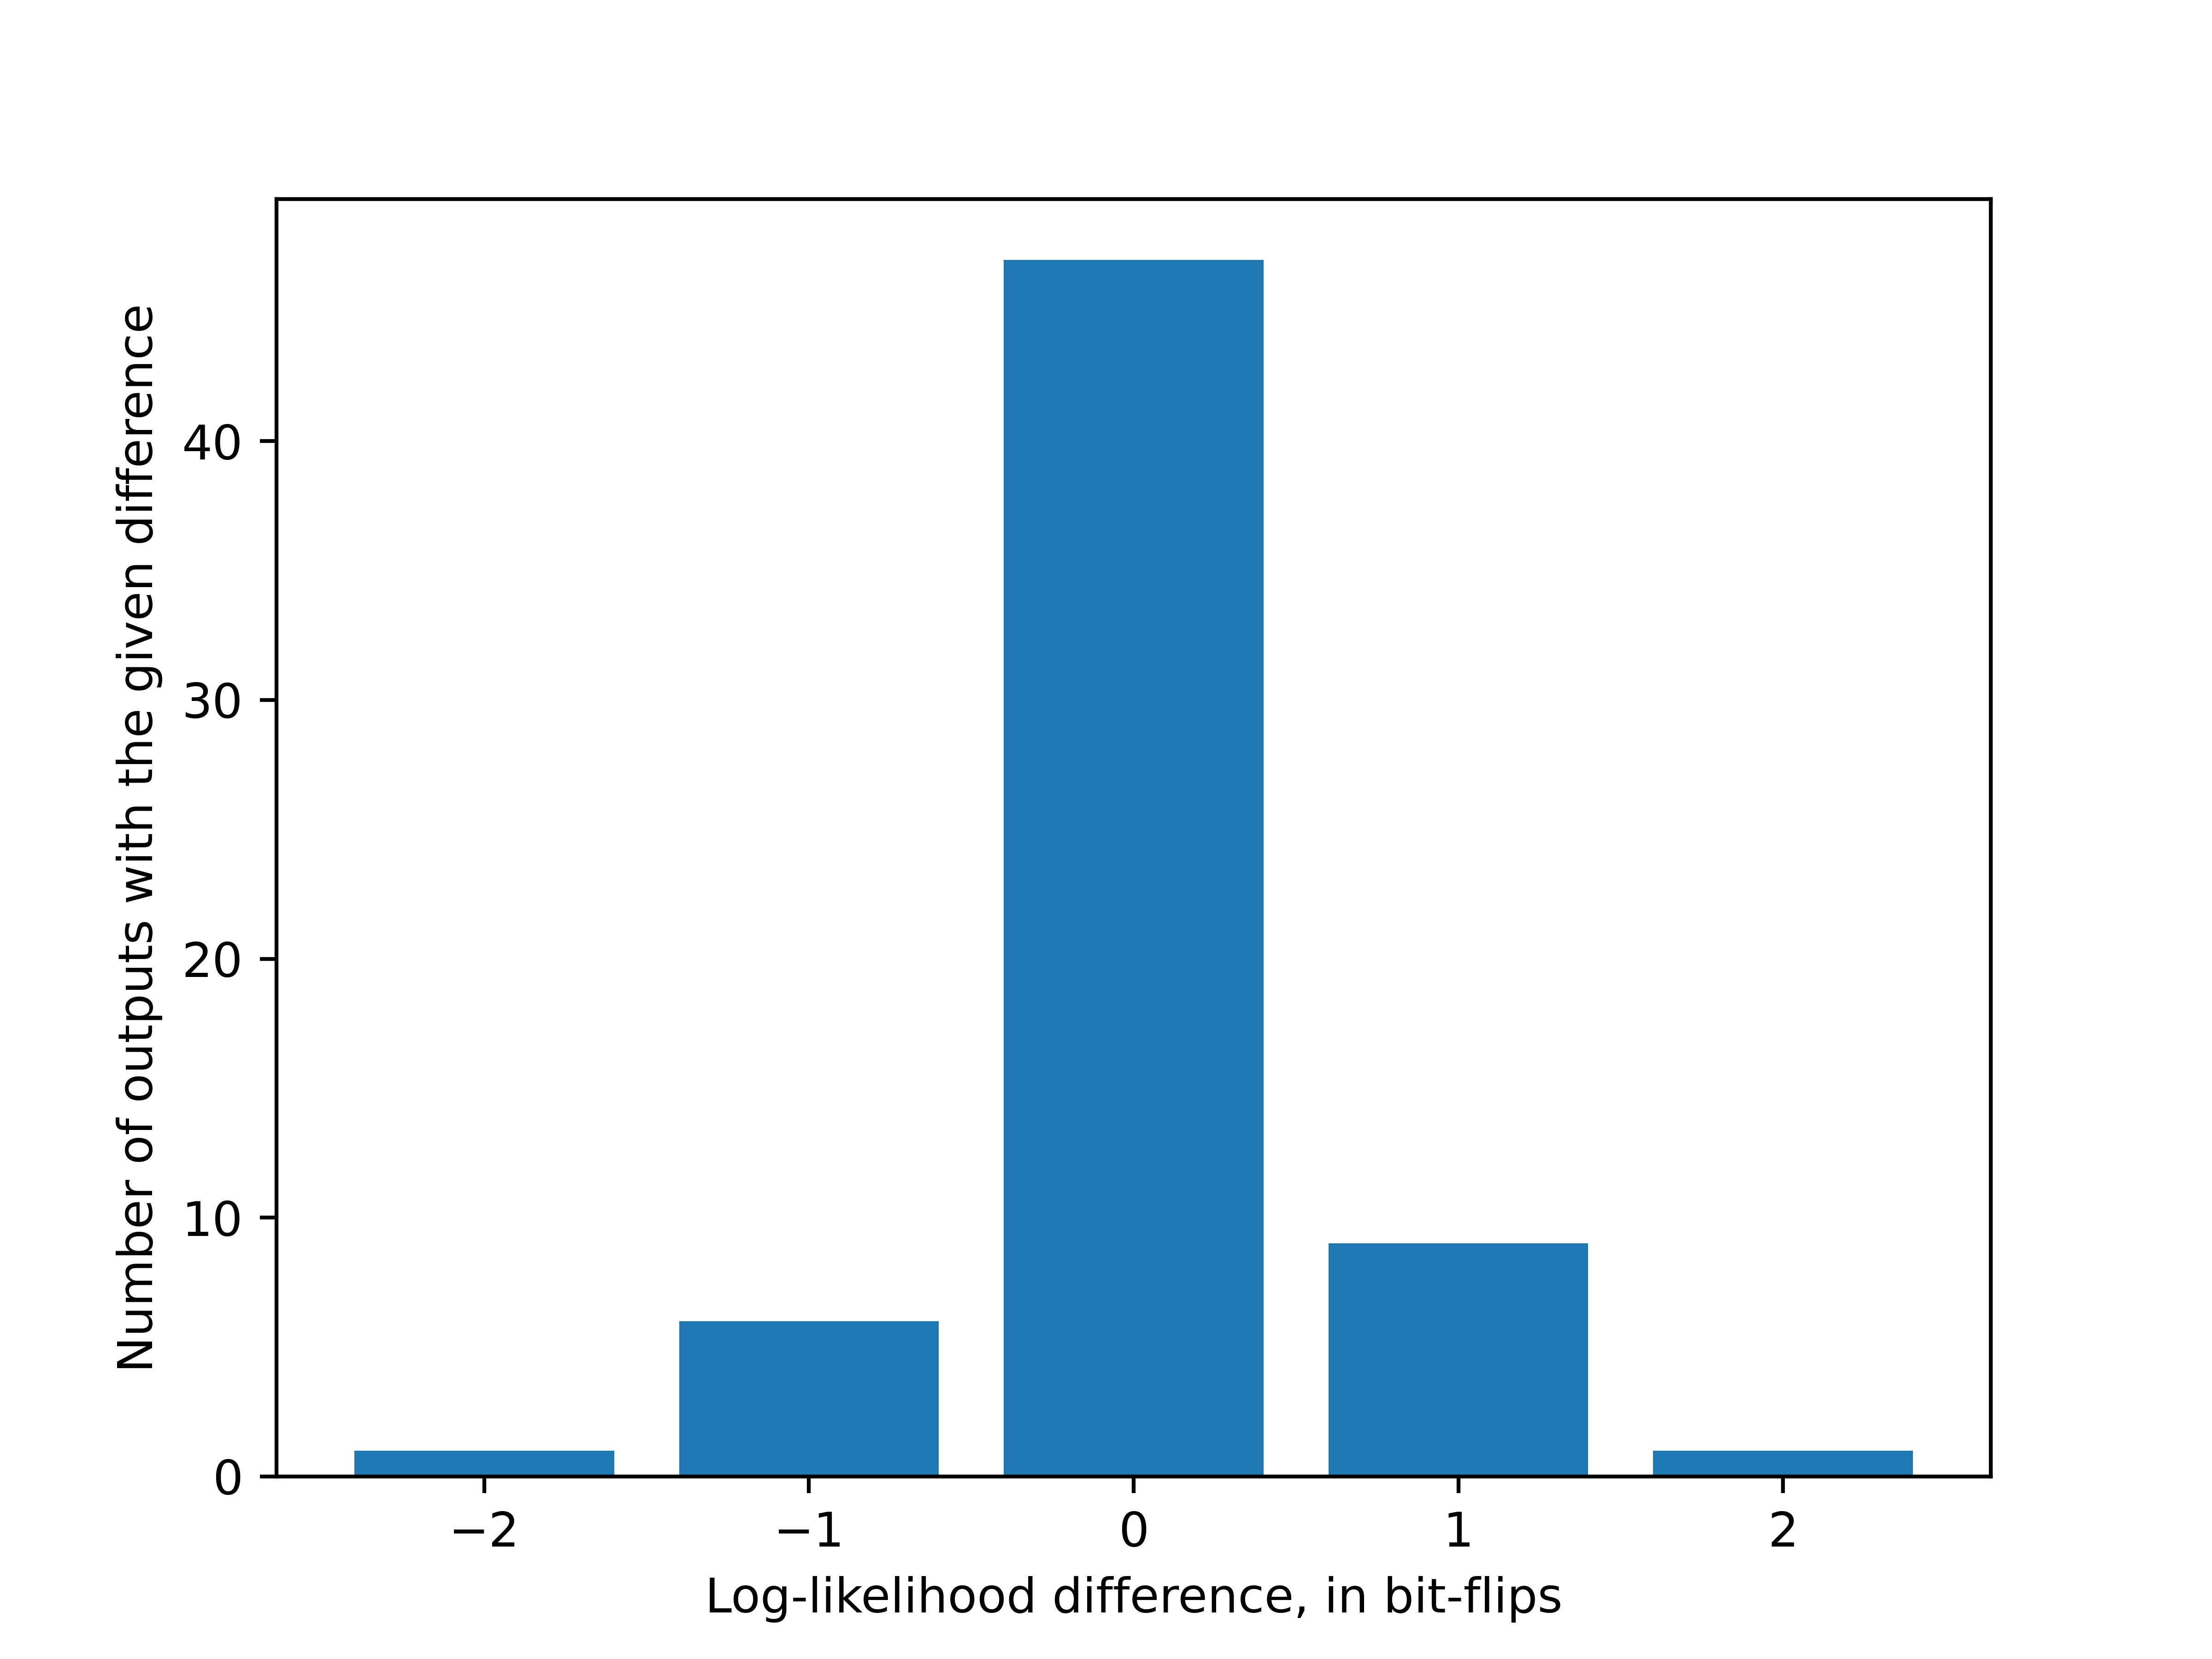
\includegraphics[width=0.75\textwidth]{figures/likelihood_differences.png}
    \caption{Accumulated differences in log-likelihood between solutions provided by \ac{SCITE} and \ac{ffSCITE}. A positive difference means that \ac{ffSCITE} has provided a better solution than \ac{SCITE}, and a negative difference means the opposite.}
    \label{fig:likelihood_differences}
\end{figure}